\documentclass[../views.tex]{subfiles}

\begin{document}

De development view laat zien hoe softwaremodules georganiseerd zijn \parencite{architectural_blueprints}. In de bovenste laag, laag vier, zijn alle packages te zien die gebruikt worden bij de beroepsproducten. Binnen een beroepsproduct worden deze ``geïmporteerd'' en ``geëxporteerd'' zodat ze bij andere packages ze kunnen aanspreken.

Elke laag is afhankelijk van de laag onder zich. In deze view is bijvoorbeeld te zien dat packages niet mogelijk zijn zonder de programmeertalen, en kunnen de programma's die in de programmeertalen geschreven zijn niet uitgevoerd worden zonder de ondersteunende software die de besturingssystemen bieden.

Aan de zijkant van de tabel zijn pijlen te zien die aangeven welk deel van de lagen domeinafhankelijk en domeinonafhankelijk zijn. Domeinonafhankelijke lagen kunnen hergebruikt worden voor andere programma's, terwijl domeinafhankelijke lagen specifiek zijn voor het omschreven product. Proxmox wordt bijvoorbeeld gebruikt om virtuele machine's voor andere programma's binnen Voys te besturen.

\begin{figure}[ht]
  \centering
  \fbox{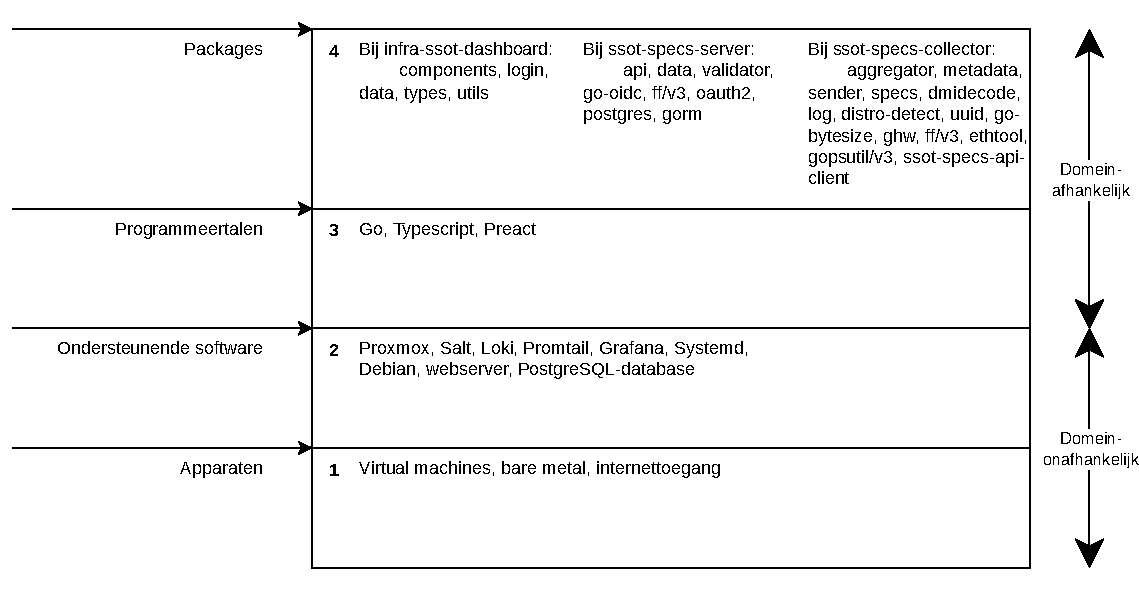
\includegraphics[width=0.95\textwidth]{../assets/images/drawio/development view.pdf}}
  \caption{De development view.}
  \label{fig:development_view}
\end{figure}

\begin{figure}[ht]
  \centering
  \fbox{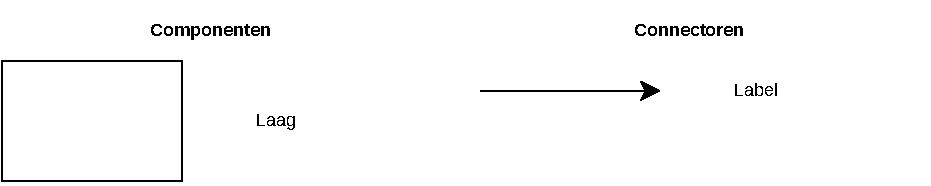
\includegraphics[width=0.95\textwidth]{../assets/images/drawio/development view legend.pdf}}
  \caption{Legenda voor \autoref{fig:development_view}.}
  \label{fig:development_view_legend}
\end{figure}

\end{document}
